%%%%%%%%%%%%%%%%%%%%%%%%%%%%%%%%%%%%%%%%%%%%%%%%%%%%%%%%%%%%%%%%%%%%%%%%%%%%%%%%
%2345678901234567890123456789012345678901234567890123456789012345678901234567890
%        1         2         3         4         5         6         7         8

\documentclass[letterpaper, 10 pt, conference]{ieeeconf}  % Comment this line out
                                                          % if you need a4paper
%\documentclass[a4paper, 10pt, conference]{ieeeconf}      % Use this line for a4
                                                          % paper

\IEEEoverridecommandlockouts                              % This command is only
                                                          % needed if you want to
                                                          % use the \thanks command
\overrideIEEEmargins
% See the \addtolength command later in the file to balance the column lengths
% on the last page of the document



% The following packages can be found on http:\\www.ctan.org
\usepackage[utf8x]{inputenc} %for linux 
%\usepackage[UTF8]{inputenc} %for windows
\usepackage{graphics} % for pdf, bitmapped graphics files
%\usepackage{epsfig} % for postscript graphics files
\usepackage{graphicx}
\usepackage{mathptmx} % assumes new font selection scheme installed
%\usepackage{times} % assumes new font selection scheme installed
\usepackage{amsmath} % assumes amsmath package installed
\usepackage{amssymb}  % assumes amsmath package installed

\usepackage{algorithm}
%\usepackage[options]{algorithm2e}
\usepackage[linesnumbered,lined,boxed,commentsnumbered,ruled]{algorithm2e}
\usepackage[noend]{algpseudocode}
\usepackage{float}
\usepackage{cases}
\usepackage{xcolor}

% If your conference documentclass or package defines these macros,
% change these macros to different names.
\newcommand*{\affaddr}[1]{#1} % No op here. Customize it for different styles.
\newcommand*{\affmark}[1][*]{\textsuperscript{#1}}
\newcommand*{\email}[1]{\texttt{#1}}

\bibliographystyle{plain}  

\title{\LARGE \bf
Learning pose constraints for trajectory optimization from demonstration}

\author{% 
Dominique M. Tao\affmark[1], Baris Akgun\affmark[2], Andrea L. Thomaz\affmark[2] and Aude Billard\affmark[1]\\\\
\parbox{3 in}{\centering \affaddr{\affmark[1]Learning Algorithms and Systems Laboratory\\
\affaddr{EPFL, Switzerland}\\
\email{\{dominique.tao,aude.billard\}@epfl.ch}\\
}}
\hspace*{ 0.7 in}
\parbox{3 in}{\centering \affaddr{\affmark[2]Socially Intelligent Machine Lab\\
Department of Computer Science \\
\affaddr{UT Austin, USA }\\
\email{athomaz@ece.utexas.edu}\\ 
}}}
\newcommand{\trsp}{{\!\scriptscriptstyle\top}}
\newcommand{\mb}[1]{{\boldsymbol{#1}}}
\newcommand{\psin}{{\!\dagger}}
\newcommand\norm[1]{\left\lVert#1\right\rVert}
\newcommand{\dosemic}{\renewcommand{\@endalgocfline}{\algocf@endline}}% Reinstate semi-colon ;
\newcommand{\pushline}{\Indp}% Indent
%\author{
%\parbox{3 in}{\centering Huibert Kwakernaak*
%         \thanks{*Use the $\backslash$thanks command to put information here}\\
%         Faculty of Electrical Engineering, Mathematics and Computer Science\\
%         University of Twente\\
%         7500 AE Enschede, The Netherlands\\
%         {\tt\small h.kwakernaak@autsubmit.com}}
%         \hspace*{ 0.5 in}
%         \parbox{3 in}{ \centering Pradeep Misra**
%         \thanks{**The footnote marks may be inserted manually}\\
%        Department of Electrical Engineering \\
%         Wright State University\\
%         Dayton, OH 45435, USA\\
%         {\tt\small pmisra@cs.wright.edu}}
%}

%\author{Dominique Tao, Baris Akgun, Andrea L. Thomaz and Aude Billard}% <-this % stops a space

%\thanks{This work was not supported by any organization}% <-this % stops a space
%\thanks{H. Kwakernaak is with Faculty of Electrical Engineering, Mathematics and Computer Science,
%        University of Twente, 7500 AE Enschede, The Netherlands
%        {\tt\small h.kwakernaak@autsubmit.com}}%
%\thanks{P. Misra is with the Department of Electrical Engineering, Wright State University,
%        Dayton, OH 45435, USA
%        {\tt\small pmisra@cs.wright.edu}}%
%}

\makeatletter
\newcommand{\removelatexerror}{\let\@latex@error\@gobble}
\makeatother

\begin{document}

\maketitle
\thispagestyle{empty}
\pagestyle{empty}


%%%%%%%%%%%%%%%%%%%%%%%%%%%%%%%%%%%%%%%%%%%%%%%%%%%%%%%%%%%%%%%%%%%%%%%%%%%%%%%%
\begin{abstract}
In the context of Keyframe-based Learning from Demonstration applied to robot manipulator, we present a framework for generating coherent trajectories with a sampling-based motion planning by using the principal direction of the constraints in the learned model. Our approach first constructs a geometric constraint of the space between two gaussians, that we call Soft-Envelope, to constrain the movement of the robot. Dimension reduction could be used on the Soft-Envelope to extract important aspects from the learned skill. Then the skill is reproduced by using our RRT* sampling-based motion planner. It generates a trajectory  w.r.t to the Soft-Envelope by using a double sampling approach combined with a natural gradient descent projection and jacobian in order to interleave between C-space and workspace. With this process, tree grows in C-space by using only samples inside a subset corresponding to the Soft-Envelope in workspace. \\
Our algorithm is tested with a 6-DOF Kinova Jaco robotic arm in simulation to get results of its performance. The skill is learned with kinesthetic teaching, and during the execution, new unseen obstacles are introduced to hinder the movement.
\end{abstract}


\begin{keywords}
 keyframe-based Learning from Demonstration approach (KLfD), sampling-based motion planning, geometric constraints (Soft-Envelope), dimension reduction, natural gradient descent projection.
\end{keywords}
%%%%%%%%%%%%%%%%%%%%%%%%%%%%%%%%%%%%%%%%%%%%%%%%%%%%%%%%%%%%%%%%%%%%%%%%%%%%%%%%

\section{INTRODUCTION}
As robots are slowly becoming more and more present in our life, one of the ultimate goal will be to have them being able to automatically and autonomously help a person, if not completely replace him, in his every daily tasks.   
While it is very tedious and complex to pre-program a specific skill for a given task that can adapt several scenarios, the Learning from Demonstration (LfD) paradigm is an widely used alternative that enables the robot to learn and generalize a skill to reproduce by observing the performance of an user.\\
In our framework, we focus on improving the creation and execution of a skill that the robot learned by using data collected from kinesthetic teaching, a common approach in LfD in which the user provides demonstrations by physically guiding the robot when performing a task as shown in figure \ref{Pic_kinesthetik_teaching}. The nature of the demonstrations that will be used consist of keyframes, which are a sparse set of sequential points in space\cite{refKeyframe1} \cite{refKeyframe2}\cite{refKeyframe0}.
A model of the skill is then constructed by clustering the keyframes in a statistical way, which can be seen as a set of constraints (position and orientation) that are used to execute the desired skill when connected in a correct sequential order. \\

\begin{figure}[ht]
	\centering
	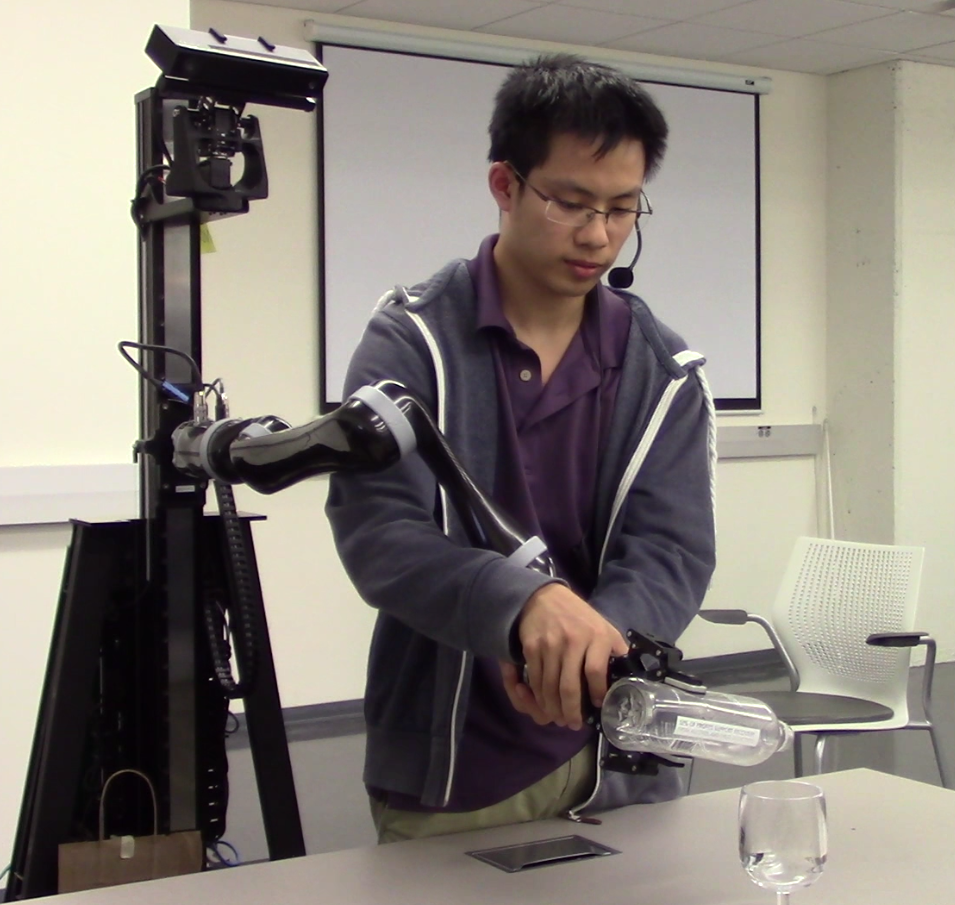
\includegraphics[scale=0.245]{figure/kinesthetic_teaching.png}
	\caption{A teacher using kinesthetic teaching with a 6-DOF Kinova Jaco arm to demonstrate a pouring water skill}
	\label{Pic_kinesthetik_teaching}
\end{figure}

Although using a spline to link the clusters together is a viable option in order to reproduce the skill \cite{refKeyframe1}, it may not be really robust when coping with a changing environment in which new obstacles that were not seen during the teaching could hinder the execution.
One attempt to solve this issue was proposed by Andrey Kurenkov \textit{et al.} in \cite{refCKframes}, in which he introduced an interactive GUI interface with the concept of Constrained-Keyframe (C-Keyframes), enabling the possibility for the user to view, edit or correct the skill model, and hence enabling a more efficient way of using a motion planning algorithm to deal with new obstacles and also having a more robust and coherent execution w.r.t the task.
However, modifying the model skill for a new constrained scenario also means that it requires the intervention of the user. %Moreover, it could also affect and bias the execution when modifying the model if more variance/freedom is added to other directions, possibly making the movement less coherent w.r.t a given task.\\

In this work, we are interested in having the robot create a more coherent motion w.r.t to its task while being able to autonomously cope with new constrained environments. Our goal is then twofold: 1) to be able to avoid, without the intervention of the user, new static obstacles that were unseen during the teaching while satisfying the model constraints 2) making the execution more coherent with the demonstrated task, ie by first trying to move and avoid obstacles along the direction that is the most relevant to the task before trying the others.\\
An illustrative example could be a scenario where the robot was given the task to fill a glass with a bottle of water that it is holding in its end-effector. Naturally, in order to succeed the task, the bottle must end up above it but it can move more freely in the vertical direction. Hence, if an object was to obstruct the execution midway, the most relevant direction to try first in order to avoid it would be the vertical axis w.r.t to the glass before trying the others depending on the height of the obstacle.\\
If demonstrations were correctly performed by the user in this perspective, clusters of the model could clearly display the information of the direction with the biggest variance. However, as shown in previous work \cite{refKeyframe2} \cite{refKeyframe0}, end-users tend to focus more on completing (\textit{what to do}) the task rather than providing good demonstrations (\textit{how to do}).\\
In order to encapsulate these different directions, we will push the analysis and dependence with the skill model further with geometric constraints and dimension reduction technique. A sampling-base motion planner will be used to deal with obstacles. 
\subsection{Proposed Approach}

The approach that we propose in this paper can essentially be divided in three parts: learning, constrained manifold creation plus possibly dimension reduction and motion planning.\\
 After collecting keyframes demonstrations with kinesthetic teaching, a skill model is created by clustering keyframes data in workspace. The clusters, in this work, are multivariate gaussians which can specify position and orientation constraints for the end-effector.\\
While the keyframes clusters are efficient to encapsulate the essence of the skill, there is no information on how the motion should be executed between two clusters, as they are sparsely distributed in space. To solve this issue and also for the used of the incoming motion planning algorithm, we constructed a "Soft-Envelope" between the two considered gaussians, named so because it designs an area in which we expect the motion of the end-effector to be. Dimension reduction method could be applied on the Soft-Envelope, resulting in a "Reduced Soft-Envelope" which will make the planner focus more on the direction with the most variance along the Soft-Envelope in order to execute the skill.  \\
The creation of the trajectory is then handled by our sampling-based motion planner, which is an extended version of the RRT* planner.
Our motivation to use such an algorithm lies in its abilities to efficiently find a feasible and collision-free path by growing a tree in space with an iterative sampling and without the user intervention. Furthermore, RRT* is probabilistically complete and asymptotically optimal if the sampling and the growth of the tree are done in the configuration space (C-space) of the robot, meaning that the planner is guaranteed to find a solution, if it exists, and that is optimal as the number of samples approaches infinity.
As we are interested in the completeness and optimality of RRT*, our planner uses a double sampling process in order to explore the C-space while trying to have its tree growing in the Soft-Envelope. Natural gradient descent and jacobian are used to switch between both spaces, enabling the creation of a series of projected points that we leverage to construct the tree in C-Space while trying to satisfy the constraints defined by the Soft-Envelope in workspace.\\

\subsection{Related Works}
Planning trajectories in the real world has always been a challenging task in robotics as for example executing the learned task in different environments.\\
 One way to create a path is to use a regression technique with a learned model of a skill as introduced by Sylvain \textit{et al.}  with the widely used GMM-GMR  w.r.t to a given environment \cite{SylvainLearningGeneralizing} (and more recently with TP-GMM as a new way to encode the data in \cite{Calinon15}) . A Similar work can also be found in \cite{refKeyframe1} by Baris \textit{et al.} using spline interpolation in a keyframes demonstration work. However, it often requires the same obstacles to be present during both the teaching and the execution of the task.\\
 Though our method also used a skill model to represent the constraints of the task, we used in addition an extended version of the RRT* to deal with obstacles. RRT* is an asymptotically optimal sampling-based motion planning algorithm introduced by Karaman \cite{KaramanRRTStar} which is a variation of RRT (Rapidly-exploring Random Trees)\cite{Lavalle98rapidly-exploringrandom} introduced by LaValle. During these past decades, a lot of literature have emerged around these two planners applied to robotics, as they allow to efficiently plan an end-to-end, collision-free trajectory in high-dimension.\\
Even though they are not using the motion planner with LfD technique, Shkolnik \textit{et al.} proposed in \cite{PathPlanningIn1000} to grow a tree in task-space by direct sampling in this same space. Though it can achieve fast planning in very high dimension, the algorithm may not be complete because the grow of the tree is only done in workspace, ignoring the collision checking in C-space during the process.  The planner RRT-JT, proposed by Vandeweghe \textit{et al.} in \cite{Vandeweghe_2007_5981} is a nice alternative to explore the workspace while checking collision with a single tree that grows in C-space. It uses the jacobian to bias the growth of the tree toward a pose in workspace by calculating the least-square solution of the error pose.
 While RRT-JT is used to explore the workspace with direction biasing, it only uses a subset of the possible joints configuration given by the least-square solution possibly making it non complete. In our work, we are exploring the full C-space with our algorithm by using the jacobian combined with projection and sampling techniques. Though the growth of our tree is influence by the sample in workspace, enough to be constrained around an area, it is not bias toward the sample itself. \\
 Berenson \textit{et al.} have done a lot of work, that have a lot in common with ours, with a single and (mainly) double complete RRT tree(s). In \cite{Berenson_WGR}, they introduced the concept of workspace goal region (WGR) to
specify goal end-effector poses that are sampled inside. Then they used an IK solver to grow their double tree IKBiRRT in C-Space.
 Difficulties of the IK and Jacobian methods were also pointed out by Bertram \textit{et al.} in \cite{Bertram_2006_5436} who bypassed them by proposing a RRT that integrates the IK solution directly in the planner by adopting workspace heuristic functions that implicitly define goal regions of the configuration.
In our work, we decided to use the jacobian instead of the IK solver, allowing our algorithm to be generalized for manipulator with more than 6 DOF where the IK solver might have  encountered problems with infinite solutions for a given pose.
Berenson \textit{et al.} also work on a planner using projection technique such as in \cite{Berenson_ConstraintManifold} in which he projects a joint angles on a constrained manifold in C-space or with the  GradientT-RRT in \cite{Berenson_Gradient}, which searches toward lower cost regions to explore. The proof of completeness of RRT-based planner using sample-project method with Jacobian is given in \cite{Berenson_2010_6558}. Task Space Regions, along with workspace goal regions, are often used in order to represent the pose constraints for the projection in his sample-project method \cite{BerensonTSR}. An other variation of projection method used with an RRT planner was also proposed by  Mike Stilman in \cite{RGD_RRT} with its RGD(random gradient descent)-RRT. Unlike their methods which are mostly projection of the joint configuration onto some constrained manifold,  we are instead using a projection onto our constrained area in workspace with a double sampling and jacobian to guide the joint configuration in C-space.
In addition, even though our constrained area can be related to their concept of Task-Space or Workspace goal region, the Soft-Envelope is more close to the representation of a prolate hyperspheroid area described in \cite{informedRRTStar} proposed by Gammell \textit{and al.} used to constrain sampling or to the Canal Space in \cite{CanalSpace} proposed by Chernova \textit{et al.}mused to encode demonstrations in order to learn a skill model.\\
Other work that combined Learning from demonstration ideas with sampling-based planning performance was done by Jonathan Classens in  \cite{RRTandLFD}, in which he used a RRT with a model learned with GMM from trajectory data collected with kinesthetic teaching. The gaussians of the model are used for direct sampling in workspace and an IK solver is used to grow the Tree in Cspace. Bowen \textit{et al.} in \cite{ModelAndPRM} also proposed a method using PRM, an equivalent planner as RRT, with a model skill encoded by clusters motion features which are a similar concept as the keyframes clusters.\\
Dimension reduction is also used to encapsulate the variation of the data to help our planner to create a more coherent trajectory w.r.t the learned task. To the best of our knowledge, only a few work have been done using dimension reduction method with a sampling-based planner.  
In \cite{balancing_statespace_coveragePCA} proposed by Yanbo \textit{et al.}, PCA is executed on all the nodes of the tree to bias its expansion toward the principal dimensions that the RRT algorithm would least explore. A similar work was done by Dalibard \textit{et al.} in \cite{PCARRT2}, in which he used PCA applied on the nodes of the RRT tree in order to find the random direction towards which the roadmap is extended. This technique is used to influence the generation of the new sample, favoring the direction along which the variance of the roadmap is high. Rosell \textit{et al.} also used PCA in \cite{PCA_PRM} over all the samples of the PRM to enlarge the probability of finding collision-free samples
in difficult regions of the C-space with low clearance.
 In our work, we use eigenvalues and eigenvectors decomposition on all the gaussians of the Soft-Envelope to determine where the variance is supposedly high along the constrained area. This new reduced area will then be used for sampling.

\section{Method Analysis}
In the following section, we will briefly consider how the model is learned from keyframes data demonstration. This model will provide as an output an ordered sequence of multivariate gaussians to recreate the skill. The algorithm, presented in the next sections, will be used by only considering two connected gaussians from the given sequence to create a local trajectory, respectively named the "parent" and "child" gaussian. The full trajectory used to recreate the task can easily be generated by combining all the local trajectories together.
\\
Let $q \in \mathbb{R}^{M \times 1}$ a joint configuration in C-Space of dimension $M$  and $p \in \mathbb{R}^{N \times 1}$ a pose in workspace of dimension $N$. $\Sigma_{p} , \Sigma_{c} \in \mathbb{R}^{N \times N}$  and $\mu_{p} , \mu_{c} \in \mathbb{R}^{N \times 1}$ respectively the covariance and center of the parent and child gaussian.\\
The different parts of the algorithm that will be explained are mainly summarized in the pseudo-code of algorithm \ref{planning}. 
\begin{algorithm}[H]
 \caption{Planning($\Sigma_p,\mu_p,\Sigma_c,\mu_c,\alpha$)}\label{planning}

\SetKwData{Left}{left}\SetKwData{This}{this}\SetKwData{Up}{up}
\SetKwFunction{Union}{Union}\SetKwFunction{FindCompress}{FindCompress}
\SetKwInOut{Input}{input}\SetKwInOut{Output}{output}
\Output{Local trajectory from parent to children gaussian}
\BlankLine
\setcounter{AlgoLine}{0}§
$V \leftarrow \{
q_{start}\}$;

$E \leftarrow \emptyset$;

$X_{sol} \leftarrow \emptyset$;

$G=(Q_q,Q_p,E,Q_{sol})$;
\BlankLine
$[\Sigma_{envSet},\mb{\mu_{envSet}}] \leftarrow$ Soft\_Envelope($\Sigma_p,\mu_p,\Sigma_c,\mu_c$);

$\Sigma_{redEnvSet} \leftarrow$ Reduced\_Soft\_Envelope($\mb{\Sigma_{envSet}}$,$\mb{\Sigma_{p}}$,$\mb{\Sigma_{c}}$, $\alpha$);

\BlankLine
PCTC\_RRTStar($G$,$\mb{\Sigma_{envSet}}$,$\mb{\Sigma_{redEnvSet}}$,$\mb{\mu_{envSet}}$, $\alpha$);

\end{algorithm}
For our variation of the RRT* algorithm, we have $T=(Q,E,Q_{sol})$ with $Q \subset Q_{free}$ the set of all vertices in C-space, the edges $E \subset Q_{free} \times Q_{free}$ and $Q_{sol}$ the set of joints configuration inside the child gaussian, used to indicate that a path is found. The set $Q$ is actually a double set $Q_q$ and $Q_p$ which respectively store the joint configuration used to grow the tree in C-space and also its pose in workspace. $\alpha$ is a parameter used as the percentage of data to be represented in the dimension reduction technique. $q_{start}$ is either the initial joint configuration of the robot or the last joint of the local trajectory solution from the previous pair of gaussians. 

\subsection{Learning - Clustering}
Should I write it, will probably refer to one paper and quickly write down how I cluster in a simple way the keyframes...
This paper suppose to show the trajectory creation so USELESS TO WRITE THAT MUCH HERE
Simple reference a comment j'ai encoder les trajectoire avec k-mean initialisation et E-M  (for chaque keyframes ==> variance is better encapsulated)
RESULTAT:
give back a simple 
\subsection{Calibration}
\subsubsection{Child and Parent Gaussian}\leavevmode\par
For a given initial pose $p_{init}$ of the robot arm, the first step is to know which pair of connected clusters to consider as parent and child gaussian for our planner.\\
We calculate the euclidean distance from $p_{init}$ to each center of all the gaussians from the given sequence and then select the gaussian $G^s$ that gives the minimal distance.
Since $G^{s}$ is from a sequence of ordered gaussians, it is at least connected to a previous $G^{s-1}$ and next gaussian $G^{s+1}$.  The euclidean distances from the pose $p_{init}$ to the center of $G^{s-1}$ and $G^{s+1}$, $\norm{\overrightarrow{\mb{p_{init}}\mb{\mu^{s-1}}}}$ and $\norm{\overrightarrow{\mb{p_{init}}\mb{\mu^{s+1}}}}$, are then calculated and compared to see which gaussian is to be paired with $G^s$ for the first used of algorithm \ref{planning}.\\
If $\norm{\overrightarrow{\mb{p_{init}}\mb{\mu^{s-1}}}}$ is smaller, then $G^{s-1}$ becomes the parent and $G^{s}$ the child gaussian (the same logic with  $G^{s}$ becoming the parent and $G^{s+1}$ the child gaussian if $\norm{\overrightarrow{\mb{p_{init}}\mb{\mu^{s+1}}}}$ was smaller).\\

\subsubsection{Soft-Envelope}\leavevmode\par
Since the skill is only encoded by a sparse set of keyframes multivariate gaussians in workspace, there is no telling how the arm end-effector should move between two clusters, especially when using a sampling-based motion planner which constructs a trajectory by sampling the space.\\
In order to constrain the motion between two considered multivariate gaussians, we introduced a constructed zone in-between them. However, our intention is not to have a hard-constraint of the motion of the end-effector, but most likely a region inside which we would like its trajectory to be, which is why we called it "Soft-Envelope" as shown in figure \ref{MixSoftEnvelope}.
\begin{figure}[h]
	\centering
	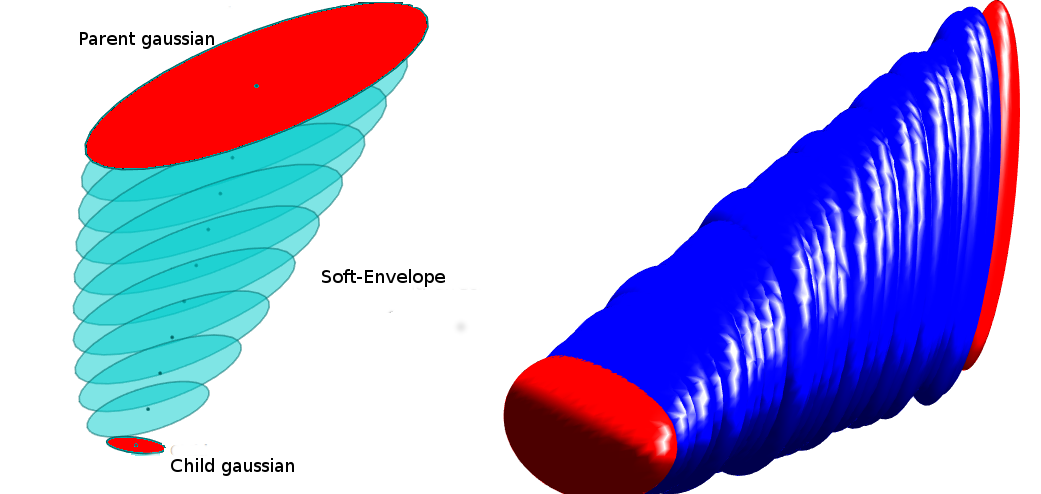
\includegraphics[scale=0.23]{figure/MixSoftEnvelope.png}
	\caption{Representation of the Soft-Envelope in 2D and 3D}
	\label{MixSoftEnvelope}
\end{figure}

The construction of the Soft-Envelope is done by linear interpolation of parent/child covariance matrices and centers as shown in the following equations: 
\begin{subnumcases}{}
			 \mb{\mu_{env}}^{0}= \mb{\mu_{p}}  \\
			 \mb{\Sigma_{env}}^{0}=\mb{\Sigma_{p}}\\
			 \mb{\mu_{env}}^{i+1} = \mb{\mu_{env}}^{i}+(\mb{\mu_{c}}-\mb{\mu_{p}})\triangle d \\
			 \mb{\Sigma_{env}}^{i+1} = \mb{\Sigma_{env}}^{i}+(\mb{\Sigma_{c}}-\mb{\Sigma_{p}})\triangle d 
			 \label{equaInterCov}
\end{subnumcases}
with $\mb{\mu_{env}}^i \in \mathbb{R}^{N \times 1}$ and $\mb{\Sigma_{env}}^i \in \mathbb{R}^{N \times N}$ the center and covariance matrix of the $i^{th}$ gaussian of the Soft-Envelope. We define $\mb{\Sigma_{envSet}}$ the set of all the calculated matrices $\mb{\Sigma_{env}}$ forming the Soft-Envelope and $\mb{\mu_{envSet}}$ the set of all $\mb{\mu_{env}}^i$ .\\ 
 Though the coefficient $\triangle d $ can be chosen as a result of a function with respect to the euclidean distance of the two center ${\norm{\overrightarrow{\mb{\mu_p}\mb{\mu_c}}}}$ , we decided instead to use a small number (w.r.t. the biggest and smallest distance between two linked gaussians in the model) since not all pair of gaussians in the model are evenly separated.\\
 
\subsubsection{Reduced Soft-Envelope}\leavevmode\par \label{ReducedSoftEnvelope}
The Soft-Envelope can also be used to encapsulate the direction with the biggest variance in each of its gaussians by using a eigenvector and eigenvalues decomposition technique, creating a "Reduced-Soft-Envelope" in full workspace. The idea is to have the end-effector move along these directions as they correspond to the linear transition between the parent and child gaussians. Furthermore, sampling will also be performed inside the (Reduced) Soft-Envelope in order to guide the creation of the trajectory.\\
The procedure is illustrated in algorithm \ref{AlgoRedSoftEnve}.\\

\begin{algorithm}[H]
 \caption{Reduced\_Soft\_Envelope($\mb{\Sigma_{envSet}}$,$\mb{\Sigma_{p}}$,$\mb{\Sigma_{c}}$, $\alpha$)}\label{AlgoRedSoftEnve}

\SetKwData{Left}{left}\SetKwData{This}{this}\SetKwData{Up}{up}
\SetKwFunction{Union}{Union}\SetKwFunction{FindCompress}{FindCompress}
\SetKwInOut{Input}{input}\SetKwInOut{Output}{output}
\Output{All $\mb{\Sigma_{red}}^i$ of the Reduced Soft-Envelope ($\Sigma_{redEnvSet}$ the set of all $\mb{\Sigma_{red}}^i$)}
\BlankLine
 \setcounter{AlgoLine}{0}

\emph{//Number of eigenvector $N_{eig}$ to represent $\alpha\%$ of the data}\;

$N_{eigP}$ $\leftarrow$ Extract\_N\_EigenDecomp($\mb{\Sigma_{p}}$, $\alpha$);\;

$N_{eigC}$ $\leftarrow$ Extract\_N\_EigenDecomp($\mb{\Sigma_{c}}$, $\alpha$);\;

\lIf{ $N_{eigC}$ $<$ $N_{eigP}$}{$N_{eig} = N_{eigP}$}\lElse{$N_{eig} = N_{eigC}$}{}
\BlankLine

\emph{//Reduced Soft-Envelope}\;


\For{$i\leftarrow $ 1 \KwTo size($\mb{\Sigma_{envSet}}$)}
{ 
	$[\mb{V}^i,\mb{D}^i] \leftarrow$ Eigen\_Decomp($\mb{\Sigma_{env}}^i$); \;
	
	$[\mb{V}_{red}^{i},\mb{D}_{red}^{i}] \leftarrow$ Reduce\_Mat($\mb{V}^i,\mb{D}^i,N_{eig}$);\;
	
	 $\mb{\Sigma_{red}}^{i} =\mb{V}_{red}^{i} \mb{D}_{red}^{i}  (\mb{V}_{red}^{i})^{\psin}$;\;
	\BlankLine
	\emph{//Calculate nearest positive definite matrix (Higmam method) and regularization }\;
	
	$\mb{\Sigma_{red}}^{i} \leftarrow$  Nearest\_PDMat($\mb{\Sigma_{red}}^{i}$);\;
	\BlankLine
	$EigVal_{Smallest} \leftarrow$ Eigen\_Decomp($\mb{\Sigma_{red}}^{i}$);\; 
	
	k=0 and $\epsilon= FLT\_EPSILON $;
	
	\While{$EigVal_{Smallest}<0$}{
	
		k++;
		
		$\mb{\Sigma_{red}}^{i}$=	$\mb{\Sigma_{red}}^{i} + (-EigVal_{Smallest} \times k^2 + \epsilon) \times \bf{I}$;
	}
}
\end{algorithm}

As a fact, one has to remember that only the parent and the child gaussians of the model truly represent the variance allowed for the task, the Soft-Envelope being just one interpretation of how the movement should be between these two. Hence, our first step will be to use eigenvalue decomposition on the child and parent gaussians to determine the biggest number of eigenvector $N_{eig}$ needed to represent $\alpha \%$ of the data, with $\alpha$ a parameter specified by the user (line 1-5). \\
We then decompose each of the Soft-Envelope gaussians covariance matrix $\mb{\Sigma_{env}}^i \in \mathbb{R}^{N \times N}$  in order to get a full eigenvector matrix $\mb{V}^{i} \in \mathbb{R}^{N \times N}$ and diagonal eigenvalue matrix $\mb{D}^{i} \in \mathbb{R}^{N \times N}$. We form the reduced  matrix $\mb{V}_{red}^{i}\in \mathbb{R}^{N \times N_{eig}}$ and $\mb{D}_{red}^{i} \in \mathbb{R}^{N_{eig} \times N_{eig}}$  by using the $N_{eig}$ biggest eigenvectors and associated eigenvalues in order to represent $\alpha \%$ of the data.
The full reduced covariance matrix from $\mb{\Sigma_{env}}^{i}$ is finally calculated with $\mb{\Sigma_{red}}^{i} =\mb{V}_{red}^{i} \mb{D}_{red}^{i}  (\mb{V}_{red}^{i})^{\psin}$, such that $\mb{\Sigma_{red}}^{i}  \in \mathbb{R}^{N \times N} $  is the covariance matrix of the $i^{th}$ gaussian of the Reduced Soft-Envelope (line 6-10). Each new reduced covariance matrix belongs to the set $\Sigma_{redEnvSet}$. A visual representation is shown in figure \ref{100vs90EnvOnly}.
\begin{figure}[h]
	\centering
	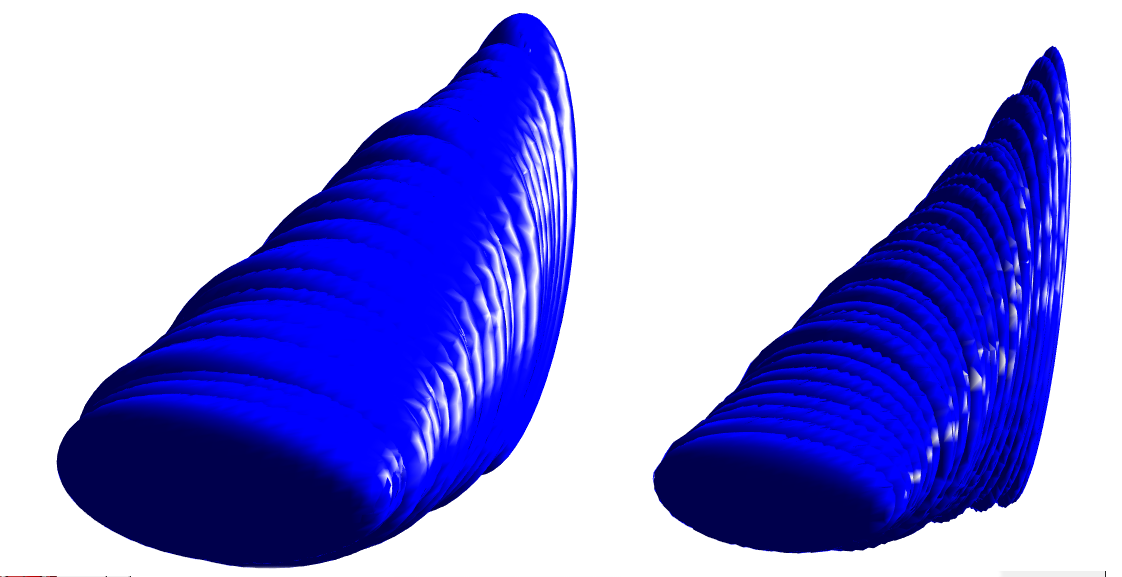
\includegraphics[scale=0.21]{figure/100vs90EnvOnly.png}
	\caption{Representation of (left image)the Soft-Envelope ($\alpha = 100$) and (right image) Reduced-Soft-Envelope($\alpha = 90$)}
	\label{100vs90EnvOnly}
\end{figure}


One particular aspect to be cautious with the gaussians of the Reduced Soft-Envelope is to make sure that they are still semi-positive definite. In fact, $\mb{\Sigma_{red}}^{i}$ being calculated by approximation of eigenvectors and eigenvalues matrices can have approximation of very small values making it just not positive definite. Since they will be later used to calculate a quadratic distance (Mahalanobis distance), it is important to have them positive definite.\\
One way to correct this problem is to use the method introduced by Higham in \cite{Nearest_PSDMATRIX} to calculate the nearest symetric semi-definite positive matrix that we can combine with a Tikhonov Regularizazion using the smallest eigenvalue if the matrix is still not positive definite (line 12-18).

\subsection{PCTC-RRT*} 
Since we are using a projection method and double sampling in both the  task-space and C-space,  we decided to name our algorithm PCTC-RRT* (Projection in Constrained Taskspace/CSpace-RRT*). PCTC-RRT* is an extension of the RRT*, ie it uses the same structure as an RRT* with some minor modification (see subsection \ref{coreRRTstarChapter}). The work was more focus on how the sampling needed to be considered w.r.t to the Soft-Envelope. The pseudo-code of the procedure is presented in the algorithm \ref{PCTCRRT}.\\
Our objective is to grow a single Tree in C-space while trying to be constrained inside the Soft-Envelope. For that purpose, we use a double sampling, one sample in each space, that we combined with a natural gradient descent projection.
The first sampling $p_{sRef}$ (line 3) is done inside the Soft-Envelope in Workspace. It is then used as the reference sampling pose on which $p_s^j$ is projected, where $p_s^j$ is the corresponding pose of the second sample $q_s$ (line 7-8).

During the projection process(line 10-33), preprocessing steps with the natural gradient is used to iteratively calculate the next pose $p_s^{j+1}$ toward $p_{sRef}$  (line 15-21). We then feed-forward the previous pose $p_s^{j}$ to have a first error $e1=p_s^{j+1} - p_s^{j}$ and also use the pose of the end-effector calculated from the previous natural gradient update, $p_{sEef}$ (line 9 or 27), as a feedback to have a second error $e2=p_s^{j+1} -p_{sEef}$ (line 22-24). The sum of them, $e=e1+e2$, is used with the Jacobian, $J$, which is calculated with the joint configuration $q_s$ in order to update this same joint configuration with the discrete Euler formula. Forward kinematic is then used to find the next pose of the end-effector $p_{sEef}$(line 25-27). When $p_s$ is projected on $p_{sRef}$, we use the new updated joint angles $q_s$ to grow the RRT* tree (line 29-32).A representation of the process can be visualized with a block diagram in figure \ref{loopControl}.\\

\begin{figure}[h]
	\centering
	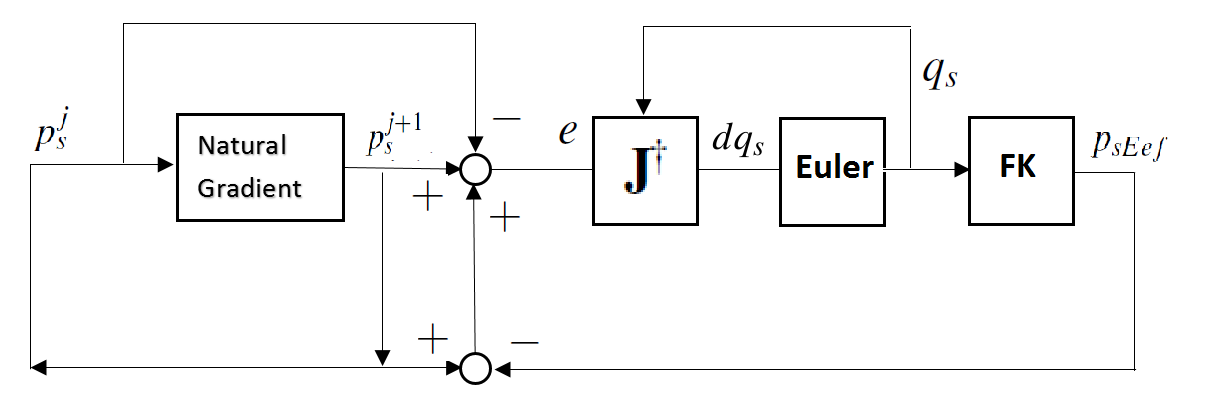
\includegraphics[scale=0.35]{figure/loopControl.png}
	\caption{Block diagram of the projection process}
	\label{loopControl}
\end{figure}

In more details, the feed-forward error $e1$ updates the joint configuration $q_s$ along the direction of the natural gradient projection. In the same logic, the feedback error $e2$ indicates along which direction $q_s$ should be updated to diminish the error between its pose and the pose calculated with the natural gradient. The evaluation of the algorithm is also possible without the feedback, but a small offset error will be created between $p_{sEef}$ and $p_s^{j+1}$ over the projection iterations since only the direction is feed-forwarded to $q_s$. \\
 In other words, we solve the IK problem for every sample  $p_{sRef}$ in the Soft-Envelope by using a natural gradient descent projection of poses in workspace in order to guide the second sample $q_s$ such that we find a joint configuration for $p_{sRef}$. This way of solving the IK problem, despite being a bit slow due to all these projections, allow us to have different joints configuration for a same point and thus properly explore the C-Space.\\
Furthermore, while we project the pose onto the reference inside the Soft-Envelope in workspace, we also exploit the series of created joints configuration $q_s$ whose poses $p_s^j$ are inside the Soft-Envelope to grow the RRT* tree (line 11-14).\\
{\fontfamily{qcr}\selectfont Get\_Membership\_SoftEnv()} evaluates which gaussian is the closest to the pose $p_s^j$ and if it is inside the Soft-Envelope. It calculates the mahalanobis distance from $p_s^j$  to each of its $i^{th}$ gaussians and then select the gaussian with the smallest distance. Then this gaussian is used to check if $p_s^j$ is inside the Soft-Enveloep with $(p_s^j-\mu_{env}^i)^{\trsp}(\Sigma_{env}^{select})^{-1} ((p_s^j-\mu_{env}^i)) < criteria$ . The value for the criteria is detailed in \cite{Filzmoser04amultivariate} (however more strict values can be use). In case we have $\alpha<100$, then we still used the covariance of the Soft-Envelope matrices to find the gaussian with the smallest mahalanobis distance but we use $(\Sigma_{redEnv}^{select})$ instead of $(\Sigma_{env}^{select})$ to check its belonging to the Reduced Soft-Envelope\\
\subsubsection{The core of PCTC-RRT*}\leavevmode\par \label{coreRRTstarChapter}
While the work was more focus in the sampling in PCTC-RRT*, the core of the algorithm remains almost the same as a RRT*. The algorithm \ref{Extended_RRTStar} presents the pseudo-code of a RRT* with, in red, the changes that we made.\\
New vertices and edges are added to $G=(Q_q,Q_p,E,Q_{sol})$ by growing the tree in the free C-space towards random selected states. Then a "choose parent" and "rewiring" steps are done for each new vertex such that it minimize the cost of nearby vertices in the Tree (more details can be found in \cite{KaramanRRTStar} ). In addition, every time a new joint configuration node is added to $Q_q$, we calculate its pose with forward kinematic which is added in the $Q_p$ set. \\
 The change that was made in {\fontfamily{qcr}\selectfont Nearest($G,q,p$)} (line 1) is that it finds the closest node  $p_{Nearest}$ from the set $Q_p$ to the pose $p$ by using the mahalanobis distance with the child covariance matrix $\Sigma_c$ in workspace. Since the two set $Q_q$ and $Q_p$ have the same number of node and ordered in the same way, we also get $q_Nearest$ which will be used to grow the RRT* tree.\\
 We also changed the condition to tell when a path is found (line 22-27). When a new node $q_{New}$ in C-space is added to the Tree, we use its corresponding pose $p_{New}$ (found with forward kinematic and added to $Q_p$) to calculate the mahalanobis distance to the children gaussian and evaluate its belonging. If we have $(p_{New}-\mu_{c}^i)^{\trsp}(\Sigma_{c}^i)^{-1} ((p_{New}-\mu_{c}^i)) < criteria$ (with the value for criteria as discuted just above), then a solution path from the parent to the child gaussian  is found (line 25). We can either directly update the next pair of parent/child gaussian in order to plan for the next new local trajectory or continue the sampling to find a more optimal path until the allowed time is reached or any other criterias specified by the user is met (local biasing can also be added to algorithm \ref{SoftEnv_Sampling} once a path is found as suggested by Baris \textit{and al.} in \cite{BarisRRT} in order to focus the sampling more around the best solution path)  \\
 

\subsubsection{Sampling}\leavevmode\par
The sampling that was done inside the Soft-Envelope follows the procedure illustrated by the pseudo-code in algorithm \ref{SoftEnv_Sampling}.
We use a goal biasing heuristic to sample inside the child gaussian, which can drastically change the planning speed (line 2-4). In that case, the covariance matrix used to generate samples inside the child gaussian is just $\Sigma_c$. Otherwise we sample uniformly inside the Soft-Envelope (line 4-9).  First, we randomly select a point on the axis connecting the center of the parent and child gaussian. This pose, $p_{sel}$, is then used in the function {\fontfamily{qcr}\selectfont Gauss\_Lin\_Interpol($p_{sel}$)} to calculate the covariance matrix $\Sigma_{sel}$  of the envelope gaussian with $p_{sel}$ as its center.\\
In fact, {\fontfamily{qcr}\selectfont Gauss\_Lin\_Interpol($p_{sel}$)} performs the same linear interpolation of the covariance matrix as in equation \ref{equaInterCov} with $\Delta d = \norm{\overrightarrow{\mb{\mu_p}\mb{\mu_{sel}}}}/{\norm{\overrightarrow{\mb{\mu_p}\mb{\mu_c}}}}$, with $\mu_{sel} = p_{sel}$. Limitations of the estimation of the calculation is also set by using the unit vector $\overrightarrow{U_{\mb{\mu_p}\mb{\mu_{c}}}} = \overrightarrow{\mb{\mu_p}\mb{\mu_{c}}}/\norm{\overrightarrow{\mb{\mu_p}\mb{\mu_{c}}}}$: in case we have $\overrightarrow{U_{\mb{\mu_{sel}}\mb{\mu_{c}}}} \neq \overrightarrow{U_{\mb{\mu_p}\mb{\mu_{c}}}} $, then it means that the center $\mu_{sel}$ is not in-between the two considered gaussians, ie it is outside from the perspective of the child gaussian, thus the covariance and center are set such as $\Sigma_{sel}=\Sigma_c$ and $\mu_{sel}=\mu_c$; in case of $\overrightarrow{U_{\mb{\mu_{p}}\mb{\mu_{sel}}}} \neq \overrightarrow{U_{\mb{\mu_p}\mb{\mu_{c}}}} $, then the center $\mu_{sel}$ is outside from the perspective of the parent gaussian, thus we have $\Sigma_{sel}=\Sigma_p$ and $\mu_{sel}=\mu_p$.\\
Once we have $\Sigma_{sel}, \mu_{sel}$, we then generate one sample from this gaussian. In case a dimension reduction need to be perform ($\alpha<100$), we simply reduce the gaussian $\Sigma_{sel}$ as explained in the section \ref{ReducedSoftEnvelope} with the algorithm \ref{AlgoRedSoftEnve} line (8-18) before generating the sample. 
\\

\subsubsection{Projection - Natural gradient descent}\leavevmode\par

Because we are using a mahalanobis distance w.r.t to the gaussians of the Soft-Envelope instead of an euclidean distance to update the pose $p_s^j$ for the projection, the natural gradient descent is used \cite{WhyAdaptiveGrad} to minimize the projection cost. The cost of the gradient takes into account two influences: the gaussian that the reference pose $p_{sRef}$ belongs to (that we are calling goal gaussian in this subsection) and the Soft-Envelope itself. While using only the goal gaussian is possible for the projection, integrating the influence of the Soft-Envelope will make the valley of the gradient cost function bend toward it. In other words, the line created by the projected points will be curved towards the Soft-Envelope. This behavior is desirable to speed the growth of the Tree since every joint configuration whose pose is inside the envelope is used to grow the RRT* tree (algorithm \ref{PCTCRRT} line 12-14).\\
The goal gaussian is determined with the function {\fontfamily{qcr}\selectfont Get\_Membership\_SoftEnv($p_{sRef}$)} which output the covariance matrix $\Sigma_{sRef}$ of the goal gaussian with $p_{sRef}$, used as the center of the goal gaussian.( algorithm \ref{PCTCRRT} line 6)\\
The influence of the Soft-Envelope is taken into account by first projecting the pose $p_s^j$ onto the axis created by the center $\mu_p, \mu_c$ of the parent and child gaussians with the function {\fontfamily{qcr}\selectfont Axis\_SoftEnv\_Ortho\_Projection($\mb{p}_s^j$)}, using the formula $p_{proj} = \mu_p + p_{tmpProj}$ with $p_{tmpProj}=\frac{ (\overrightarrow{\mu_p\mb{p}_s^j} \cdot \overrightarrow{\mu_p\mu_c})}{\norm{\overrightarrow{\mu_p\mu_c}}^2}\overrightarrow{\mu_p\mu_c} $ \\
The projected point $p_{proj}$ on the axis is then used in the function {\fontfamily{qcr}\selectfont Gauss\_Lin\_Interpol($p_{proj}$)} to find the center $\mu_g^j$ and covariance $\Sigma_g^j$ of the gaussian inside the Soft-Envelope that will influence the gradient cost function (algorithm \ref{PCTCRRT} line 15-16).\\

One has to notice that $p_{sRef}$ which is not necessarily on the axis of the parent-child center was chosen as the center for $\Sigma_g$, creating an offset in the projection. In order to correct it, the same orthogonal projection function is used on the reference sample $p_{sRef}$ to calculate this "offset" which will be added to  $\mu_g^j$ before it will be used in the natural gradient update(algorithm \ref{PCTCRRT} line 4-5 and 17).\\

The natural gradient is calculated by using the mahalanobis metric such as: 
\begin{equation}
			 coeff = \frac{\norm{\overrightarrow{\mu_c\mu_p}}}{(\mu_p-\mu_c)^{\trsp}\Sigma_c^{-1}(\mu_p-\mu_c)}
\end{equation}
\begin{subnumcases}{}
			 F_{Goal}=(p_s^j - p_{sRef})^{\trsp}\Sigma_{sRef}^{-1}(p_s^j - p_{sRef}) \\
			 F_{Env}=(p_s^j - p_{proj}^j)^{\trsp}\Sigma_{g}^{-1}(p_s^j - p_{proj}^j)
\end{subnumcases}
\begin{subnumcases}{}
 			dF_{Goal}=2\Sigma_{sRef}^{-1}(p_s^j - p_{sRef}) \\
			dF_{Env}=2\Sigma_{g}^{-1}(p_s^j - p_{proj}^j)
\end{subnumcases}
The update of $p_s^j$ is done with :
\begin{equation}
	p_s^j = p_s^j+\delta_{n}(\Sigma_{g}(-coeff \times dF_{Env} )+\Sigma_{sRef}(-coeff \times dF_{Goal} ))
	\label{equCostNatGrad}
\end{equation}

with $\delta_{n}$ the natural gradient stepsize. \\
The choice of the stepsize is important for a correct convergence of the projection. Numerous techniques exist to calculate the stepsize of a gradient descent projection, but most of them still create too much points because of the value of the stepsize which is chosen small to avoid divergence. In addition of being slow, this might also cause an unwanted biasing of the tree growth toward some specific regions other than the child gaussian.\\
Since the goal of the projection is different for each new sample of $p_{sRef}$, we use an adaptive step-size for each new projection by using the same formula illustrated in \cite{AdaptiveStepSizeNatGrad} used in a reinforcement learning framework, p. 289 equation 6. 

\begin{subnumcases}{}
	step1 = (coeff \times dF_{Goal})^{\trsp} \Sigma_{sRef} (coeff \times dF_{Goal}) \\
	step2 =	(coeff \times dF_{Env})^{\trsp} \Sigma_{g} (coeff \times dF_{Env}) \\
	\delta_{n} = \frac{1}{\sqrt{(step1+step2)}}
	\label{stepSizeAdaptive}
\end{subnumcases}

The calculation of $\delta_{n}$ is only done once at the beginning of each new projection (ie for each new sample $p_{sRef}$), which allows a faster projection as the poses at the beginning are more distant. In fact, if the next pose updated by the natural gradient converges towards $p_{sRef}$, then the rest of the projection will also converge for the same calculated step-size because the mahalanobis distance from each new updated pose to  $p_{sRef}$ is decreasing.\\
Since the context of application of this formula is different, we implemented an additional step to avoid divergence of the projection. If the mahalanobis distance of the first updated pose $p_s^{j+1}$ is bigger than the distance of the original pose sample $p_s^{j}$, then it means that the step of the new updated pose was too big and then the projection will diverge. We corrected this problem by diminishing the step-size N times until convergence ( $\delta_{n}= \delta_{n} \times a$ with $0<a<1$, in a similar way as the step-size line search backtracking method), with N a parameter defined by the user. If after N times, the criteria is still not met, then the projection is not evaluated.

\begin{algorithm}[H]
 \caption{PCTC\_RRTStar($G$,$\mb{\Sigma_{envSet}}$,$\mb{\Sigma_{redEnvSet}}$,$\mb{\mu_{envSet}}$, $\alpha$)}\label{PCTCRRT}

\SetKwData{Left}{left}\SetKwData{This}{this}\SetKwData{Up}{up}
\SetKwFunction{Union}{Union}\SetKwFunction{FindCompress}{FindCompress}
\SetKwInOut{Input}{input}\SetKwInOut{Output}{output}

\setcounter{AlgoLine}{0}
\Input{In addition, $\Sigma_p,\Sigma_c,\mu_p$ and $\mu_c$ are assumed available for all the functions here}
\Output{Solution path connecting the parent and child gaussian}
\BlankLine
\textcolor{blue}{\emph{//First loop: creation of workspace and C-space samples,}\;}

	\While{TRUE or ALLOWED TIME}
	{
	\BlankLine
		$p_{sRef} \leftarrow $ SoftEnv\_Sampling($\Sigma_{envSet}, \Sigma_{redEnvSet},\alpha$);
		
		$\mb{p}_{projRef} \leftarrow$	Axis\_SoftEnv\_Ortho\_Projection($p_{sRef}$);
		
		$v_{offset} = p_{sRef}-\mb{p}_{projRef} $;
		\BlankLine
		$[\Sigma_{sRef},flag_{sRef}]\leftarrow$\\ Get\_Membership\_SoftEnv($p_{sRef},\Sigma_{envSet}, \Sigma_{redEnvSet}$,$\mb{\mu_{envSet}}$);
		\BlankLine
		
		$q_s\leftarrow $Random\_Real\_From0To2PI();
		
		$p_s^j\leftarrow $ Forward\_Kin($q_s$);
		
		$p_{sEef}=p_s^j$;
		\BlankLine
			
	\textcolor{blue}{\emph{//Second loop: Gradient projection and Tree growing}}
		\While{TRUE or ALLOWED TIME}
		{
			\BlankLine

			$[\Sigma_2,flag2_{belong}]\leftarrow$\\ 
			Get\_Membership\_SoftEnv($p_s^j,\Sigma_{envSet}, \Sigma_{redEnvSet}$,$\mb{\mu_{envSet}}$);
			\BlankLine
			
			\If{$flag2_{belong} == TRUE$}
			{
				
				$S_{path}\leftarrow $ Extended\_RRTStar($G,q_s,p_s$);
			}
			\BlankLine
				
			$\mb{p}_{proj} \leftarrow$	Axis\_SoftEnv\_Ortho\_Projection($\mb{p}_s^j$);
			
			$[\Sigma_{g},\mu_{g}] \leftarrow$ Gauss\_Lin\_Interpol($\mb{p}_{proj}$);
			
			$\mu_{g} = \mu_{g} + v_{offset}$;
			\BlankLine
			\BlankLine
			$[\mb{p}_s^{j+1},flag_{diverge}] \leftarrow$\\
			 Natural\_Gradient($\mb{p}_s^{j},\Sigma_{sRef},\mb{p}_{sRef},\Sigma_{g},\mu_{g}$);
			\BlankLine
			\If{$flag_{diverge} == TRUE$}
			{
			
				break;
			}
			
			$e_1=p_s^{j+1} - p_s^{j}$;
			
			$e_2=p_s^{j+1} - p_{sEef}$;
			
			$e=e_1+e_2$;
			
			\BlankLine
			$\bf{J}\leftarrow$GetJacobian($q_s$);
			
			$q_s=q_s+ \bf{J}^{\psin} e$;
			
			$p_{sEef}\leftarrow $ Forward\_Kin($q_s$);
			
			\BlankLine
			$p_s^{j} = p_s^{j+1}$
			\BlankLine
			
			\If{$p_s$ projected on $p_{sRef}$}
			{
				$G \leftarrow $ Extended\_RRTStar($G,q_s,p_{sRef}$);
				
				break;
			}
		}
	}
\end{algorithm}

\begin{algorithm}[H]
 \caption{Extended\_RRTStar($G,q,p$)}\label{Extended_RRTStar}

\SetKwData{Left}{left}\SetKwData{This}{this}\SetKwData{Up}{up}
\SetKwFunction{Union}{Union}\SetKwFunction{FindCompress}{FindCompress}
\SetKwInOut{Input}{input}\SetKwInOut{Output}{output}

\setcounter{AlgoLine}{0}

\Output{set of vertices and edges $G=(Q_q,Q_p,E,Q_{sol})$}
\BlankLine

\textcolor{red} {$[q_{Nearest},x_{Nearest}] \leftarrow$ Nearest($G,q,p$);}

$q_{New} \leftarrow$ Steer($q_{Nearest},q$);

\If{Collision\_Free($q_{Nearest}, q_{New}$)}
{
	$Q_q \leftarrow Q_q \cup  q_{New} $;
	
	$q_{Min} \leftarrow  q_{Nearest}$;
	
	$Q_{Near} \leftarrow$ Near($G,q$);
	
	\ForAll{$q_{Near} \in Q_{Near}$}
	{
		\If{Collision\_Free($q_{Near}, q_{New}$)}
		{
			\If{Cost($q_{Near}$)+CostIm($q_{Near},q_{New}$)$<$Cost($q_{New}$)}
			{
				$q_{Min} \leftarrow Q_{Near}$;
			}
			
		}
	}
	
	$E \leftarrow E \cup (q_{Min},q_{New})$;
	
	\ForAll{$q_{Near} \in Q_{Near}$\textbackslash $q_{Min}$}
	{
		\If{Collision\_Free($q_{Near}, q_{New}$) and Cost($q_{New}$)+CostIm($q_{Near},q_{New}$) $<$ Cost($q_{Near}$)}
		{
			$q_{Par} \leftarrow$ Parent($q_{Near}$); 
			
			$E \leftarrow E$ \textbackslash $(q_{Par},q_{Near})$;
			
			$E \leftarrow E \cup (q_{New},q_{Near})$;
		}
	}
    

\BlankLine
	\textcolor{red} {$p_{New}\leftarrow$ Forward\_Kin($q_{New}$);}
	
	\textcolor{red} {	$Q_p \leftarrow Q_p \cup  p_{New} $;}
	
	\textcolor{red}{ $dist\_goal \leftarrow$ MahalanobisDist($p_{New},\Sigma_{c},\mu_{c}$);}
	 
	\textcolor{red} {\If{dist\_goal $<$ GaussBelongCrit}
	{
		$Q_{sol} \leftarrow Q_{sol} \cup {p_{New}}$;
	}
	}
}
\end{algorithm}


\begin{algorithm}[H]
 \caption{SoftEnv\_Sampling($\Sigma_{envSet}, \Sigma_{redEnvSet},\alpha$)}\label{SoftEnv_Sampling}

\SetKwData{Left}{left}\SetKwData{This}{this}\SetKwData{Up}{up}
\SetKwFunction{Union}{Union}\SetKwFunction{FindCompress}{FindCompress}
\SetKwInOut{Input}{input}\SetKwInOut{Output}{output}

\setcounter{AlgoLine}{0}
\Input{In addition, $\Sigma_p,\Sigma_c,\mu_p$ and $\mu_c$ are assumed available for all the functions here}
\Output{Sample $q_s$ in C-space }
\BlankLine
 $randProb \leftarrow $Random\_Real\_From0To2PI();
 
	\uIf{randProb $<$ GoalBias}
	{
		$\Sigma_{sel} = \Sigma_c$;
	}
	\Else
	{
	 	$randNum \leftarrow $Random\_Real\_From0To2PI();
	 	
	 	$U_{axis}=(\mu_c - \mu_p)/\overrightarrow{{\mb{\mu_p}\mb{\mu_{c}}}}$;
	 	
	 	$p_{sel}=\mu_p+U_{axis}*(randNum \times \overrightarrow{{\mb{\mu_p}\mb{\mu_{c}}}})$;
	 	
	 	$[\Sigma_{sel},\mu_{sel}] \leftarrow$ Gauss\_Lin\_Interpol($p_{sel}$);
	}
	\uIf{$\alpha$ $<$ 100}
	{
		$\Sigma_{redSel} \leftarrow $ reduction $\Sigma_{sel}$ as in algorithm \ref{MixSoftEnvelope} (line 8-18);
		
		$q_s \leftarrow $ Sample\_Gaussian($\Sigma_{redSel}$);
	}
	\Else
	{
		$q_s \leftarrow $ Sample\_Gaussian($\Sigma_{sel}$);
	}
\end{algorithm}

\section{Experiments}
We use a real robot to provide demonstration and a simulated robot to emulate its behavior and get results.
We first used a real 6-dof Kinova Jaco Arm that is mounted horizontally on a robot platform as shown in figure \ref{Pic_kinesthetik_teaching} to collect keyframes data. Kinesthetic teaching was used to demonstrate the skill to the arm which was gravity-compensated. A GUI interface was utilized in order to indicate when to record the keyframe ( in joints angle (C-space) and also position-quaternion (workspace)) with the following key-phrase: "Start here" for starting the demonstration and recording the first keyframe, "Go here" to record a keyframe during the demonstration and "End here" to record the last keyframe and finish the demonstration. \\
We then evaluated our algorithm with Moveit-Rviz simulator with the learned model in Workspace as input for our algorithm written in C++. The "Eigen" C++ library was used for the linear algebra and eigenvalues/vectors decomposition. The behavior of the robot arm was tested in 2 different scenarios. The setup for each of them was with a 0.61m x 1.22m x 0.73m table on which were disposed different objects from the YCB set. Simulation was done on a Lenovo computer with  a Intel Core i7-5600U CPU 2.60GHz × 4 processor and Nvidia GeForce 940M graphic card.\\
In each scenario, the initial configuration of the arm is placed such that its end-effector is inside the first keyframes cluster, in other words the initial configuration of the arm is such that the entire arme is above the table. First, the user demonstrate a specific task to the robot in a environment without any obstacles and 10 successful demonstrations will be selected to learn the skill model. Then new obstacles will be added before the planning of the trajectory. Our objective is to evaluate how the robot perform the task by generating an end-to-end trajectory while respecting the Soft-Envelope constraints and finding the correct direction to avoid the obstacle.
NB: IN IMAGE LEGEND, SPECIFY THAT COLOR == ORDER OF CLUSTER AND ONLY REPRESENTATION IN X Y Z 3D DIMENSION WORKSPACE

\subsection{Parameters}
WRITE HERE THE VALUE OF THE PARAMETER USE FOR IN THE ALGORITHM

\subsection{Scenario 1: Pick and Place}
In this scenario, the robot was taught a pick and place skill in which it has to pick an object(more likely a fruit) and put it on a dish as shown in image METTRE IMAGE ICI. During the reproduction of the skill in simulation, OBSTACLE DESCRIPTION TO BE PUT HERE  was introduced between the initial configuration of the arm and the dish as shown in image METTRE IMAGE ICI.
 The skill model is represented by 2 keyframes clusters. For this task, the position constraints is important but not the orientation as the grasped object can be turn upside down without changing the success of the task.\\
 As we can see in image METTRE IMAGE ICI, the last cluster is wide but not tall, so we are expecting the end-effector to avoid the obstacle first by trying the x-y direction before the vertical one (w.r.t. the table)

\subsection{Scenario 2: Pouring water from bottle}
In this scenario, the robot is holding a bottle of water at its end-effector gripper. Its mission is to pour water from into bottle into a glass on the table at its opposite side.
Two type of obstacles were introduced as to study the movement of the arm: a tall but slim one DECRIRE OBJECT ICI, and a large but short one DECRIRE OBJECT ICI\\
The skill of the model is composed of 3 keyframes multivariate gaussians. The first the second gaussian describe the movement of the arm from its initial position to the area above the glass without spilling the water, the third one is superposed to the second cluster as to indicate the rotation of the end-effector to pour the water into the glass.\\
With this task, we are dealing with position and orientation constraints. In fact, during the first movement, it is important to respect the orientation constraint in order to not spill the water while avoiding obstacle, the same with the second movement during which it must remain above the glass while correctly spinning its gripper.\\

\subsection{Scenario 3: Reversing cup}
In this last scenario, the robot is holding a plastic cup DECRIRE OBJECT ICI in its gripper. With the same interest that we had for the previous scenario, the robot must perform a pick and place task by putting the cup in reverse state on a specified zone of the table while avoiding a obstacle of different heights. \\
This skill is encoded by two keyframes multivariate gaussians. The constraint follows the first scenario with the difference that the end-effector is now under position and also orientation constraints as it has to reverse the position of the cup mid-way.

\section{Results}
\section{Discussion}
  Need to see result to know how to shape this paragraph...
Discuss why results and why sometime fail (not JTRRT, our planner explore the c-space without any biasing in Workspace, so... Tree is constrained inside Soft-Envelope but not direction biasins and thus still have strength of exploration ==> good with concept of soft envelope since more change to take other direction)\\

In futur work, JT-RRT from Vend blabla is for biasing in workspace but no completeness, in our explore the C-space but not biasing ==> possibility combination\\

Other things to discuss: Completness of our algorithm not proven ==> reference to Berenson work which prove it and can be use for ours since similar\\

Optimality not proven either.

Suggestion of evolution of the parameter $\alpha$ over time, if no solution found during the allowed time, have $\alpha$ to go to 100 and consider more eigenvector and less dimension reduction and once 100 consider everything \\

\section{Future Work}
Next logical step: consider a second point of view ==> now only move according to the variance with the model skill ==> too dependent of the demonstraiton
Integration of the sitaution view from different referential (kinect for example)==> analysis of the environment ==> if obstacle too tall, even if model variance is big, maybe not sampling in this area ? ... \\
Basically Now it is still related to demonstration if demonstration fail to do so then done, integrate object to seize favorable direction.
Orientation working or not ?  Need to see result to know how to shape this paragraph...
Mettre article dans discussion pour possibilité d'amélioration:
RealTimeRRT, RRTOptimalConnect,RRTx,Anytime RRT*
Also used bi-RRT*: futur work

futur work : possibility to improve the algorithm by making it possible to deal with dynamic environment with RRTx as suggested by Otte \textit{et al.} \cite{RRTx}

\section{Conclusion}
In this paper, we have presented trajectory planning combined with a learned skill from keyframes demonstration. The concept of Soft-Envelope, a constrained area between two keyframes gaussians was proposed in which an extension of the RRT*, PCTC-RRT*, was used to find a non-collision and available configuration space path linking two considered gaussians whose correspondent poses were around/inside the Soft-Envelope. The planner interleave the exploration of C-space while being constrained in an area in workspace by using a double sampling process combined with gradient projection.
The algorithm was tested on  DOIT FINIR CA AVEC LES EXPERIMENTS ET RESULTS

\section{Acknowledgements}
The authors would like to thank Aude Billard for making this joint research possible, Andrea L. Thomaz and Akgun Baris for the time that they spent for valuable help and discussions.
%%%%%%%%%%%%%%%%%%%%%%%%%%%%%%%%%%%%%%%%%%%%%%%%%%%%%%%%%%%%%%%%%%%%%%%%%%%%%%%%

\bibliography{bible}


\end{document}
